%Revisado
\section{Viabilidade Industrial e \textit{Trade-off} Computacional (QP4)}
\label{sec:viabilidade_industrial}

Um dos desafios desta dissertação reside em equilibrar o rigor estatístico com a viabilidade operacional para o setor agroindustrial. Embora a \textbf{DenseNet (RGB/BR)} tenha alcançado a liderança em termos de MCC absoluto ($0,6461$), um modelo destinado à produção deve ser avaliado também por seu custo computacional, demanda energética e latência de inferência em tempo real.

A Tabela \ref{tab:industrial_ranking} consolida os indicadores de produtividade para os modelos treinados na melhor versão do conjunto de dados (RGB/BR). A análise revela um compromisso crítico (\textit{trade-off}) entre precisão e velocidade: enquanto a DenseNet lidera no eixo preditivo (MCC), ela apresenta uma latência de inferência de $19,04$ ms, significativamente superior à da \textbf{ConvNeXt} ($6,44$ ms). Adicionalmente, nota-se que a \textbf{EfficientNet} apresenta a maior eficiência algorítmica bruta, com apenas $0,6813$ GFLOPs, tornando-a uma candidata primorosa para dispositivos de borda (\textit{edge computing}) com extrema restrição de \textit{hardware}, ainda que com um MCC marginalmente inferior ($0,5915$).

\begin{table}[!h]
    \centering
    \begin{threeparttable}
    \caption{Ranking de Eficiência Industrial (Conjunto de Dados RGB/BR).}
    \label{tab:industrial_ranking}
    \begin{tabular}{llllll}
\toprule
Modelo & MCC & Parâmetros (M) & Tamanho (MB) & Latência (ms) & GFLOPs \\
\midrule
DENSENET & \textbf{0,6461} & 7,4838 & \textbf{29,1242} & 19,0448 & 2,8651 \\
CONVNEXT & 0,6153 & 28,3478 & 108,2258 & \textbf{6,4413} & 4,4702 \\
EFFICIENTNET & 0,5915 & 8,0643 & 31,2395 & 12,9784 & \textbf{0,6813} \\
VGG & 0,4910 & 33,0164 & 126,0395 & 11,2935 & 19,5511 \\
RESNET & 0,4501 & 24,6910 & 94,4991 & 7,8715 & 4,1106 \\
VIT & 0,4328 & 86,0297 & 328,2475 & 15,2857 & 16,8669 \\
SWIN & 0,4143 & 28,0470 & 107,2936 & 11,2551 & 4,5090 \\
INCEPTION & 0,2882 & 23,8940 & 91,4711 & 11,9814 & 2,8473 \\
\bottomrule
\end{tabular}

    \begin{tablenotes}
            \small 
            \item[] Fonte: Do autor (2026).
        \end{tablenotes}
        \end{threeparttable}
\end{table}

Para validar a robustez destes resultados, a Figura \ref{fig:p_values_v10} apresenta a matriz de significância estatística (McNemar) entre todos os modelos na versão RGB/BR. Observa-se que a superioridade da DenseNet e da ConvNext sobre arquiteturas clássicas como ResNet e Inception é estatisticamente significante ($p < 0,01$). ontudo, o teste revela que a diferença de performance entre as líderes DenseNet e ConvNeXt não é estatisticamente significativa ($p > 0,05$). Estatisticamente, isso indica um desempenho semelhante no poder de generalização de ambas as redes para este domínio.

\begin{figure}[h!]
  \centering
  \caption{Matriz de significância estatística (McNemar) no conjunto de dados RGB/BR. O sufixo (ns) indica ausência de diferença estatística significante ($p > 0,05$).}
  \label{fig:p_values_v10}
  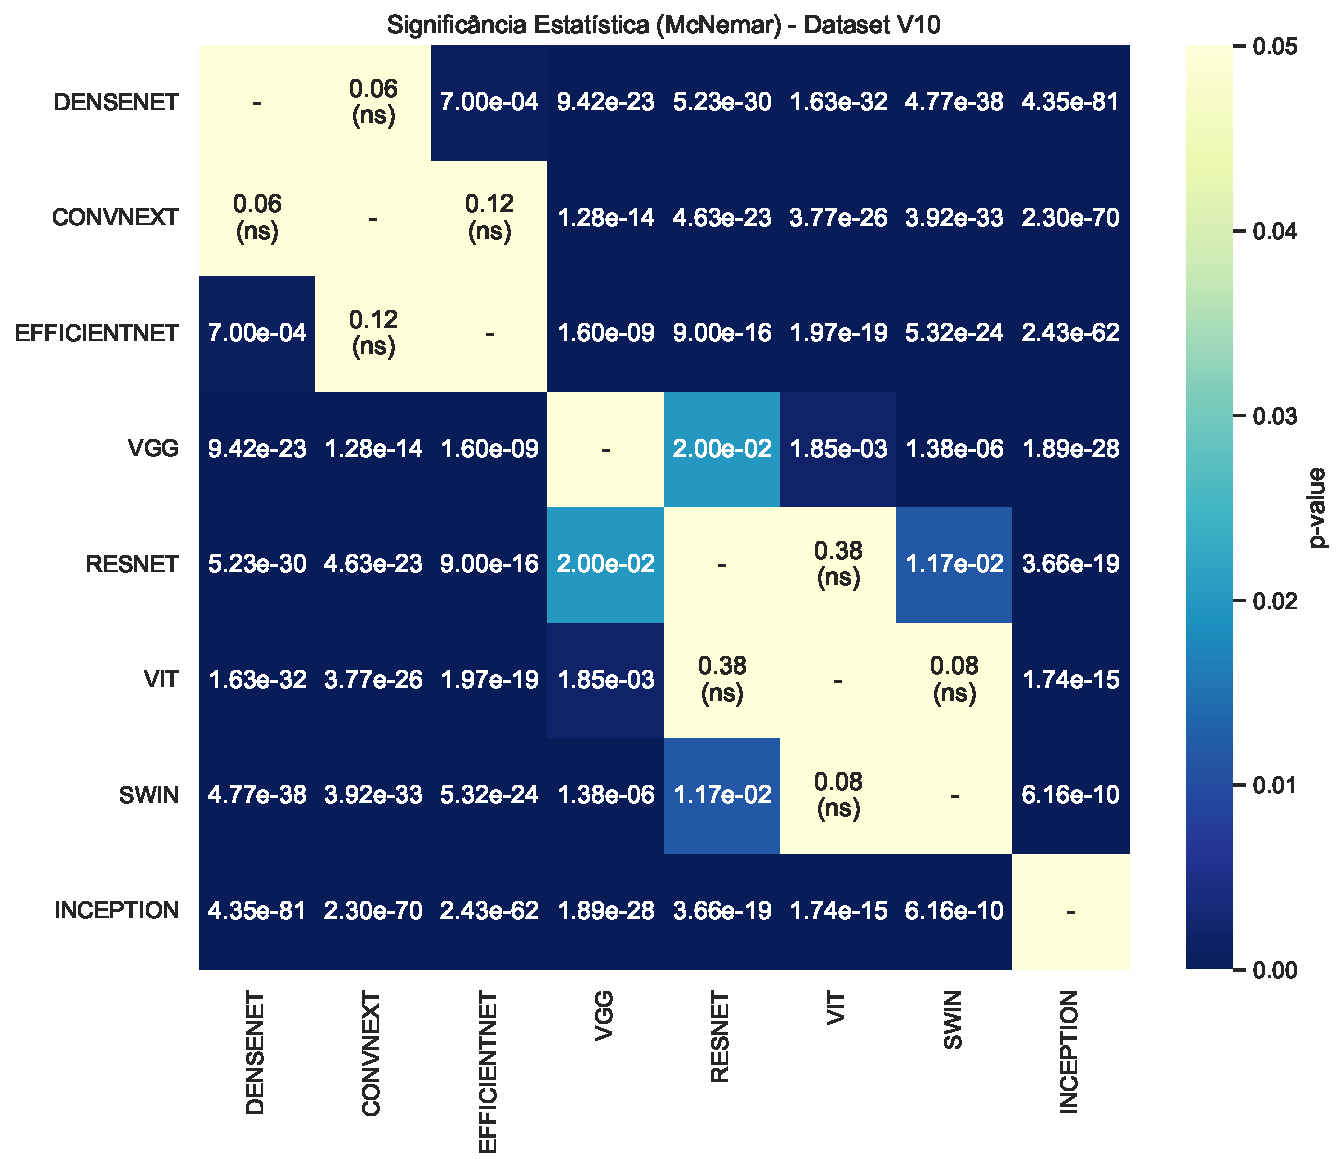
\includegraphics[width=0.8\textwidth]{images/p_value_heatmap_v10.pdf}
  \legend{Fonte: Do autor (2026).}
\end{figure}

Diante do empate na predição, o critério de seleção segue obrigatoriamente sobre as métricas de engenharia. Para visualizar este cenário, a Figura \ref{fig:efficiency_tradeoff} correlaciona o MCC com a latência de inferência, permitindo a identificação de três perfis tecnológicos distintos:

\begin{itemize}
    \item \textbf{Alta Precisão (Elite):} A \textbf{DenseNet} ocupa o topo do gráfico e surpreende pelo menor consumo de armazenamento (\textbf{$29,12$ MB}), mas seu deslocamento para a direita no eixo de latência pode limitar sua adoção em esteiras de classificação de fluxo contínuo ultra-veloz.
    \item \textbf{Sweet Spot Industrial:} A \textbf{ConvNext} emerge como a arquitetura suprema para o domínio, oferecendo performance estatisticamente equivalente à líder com a menor latência entre os modelos de alta performance. Sua agilidade, aliada a uma complexidade de \textbf{$4,47$ GFLOPs}, responde à Questão de Pesquisa QP4.
    \item \textbf{Baixa Eficiência:} Os modelos baseados em \textbf{Transformers} (bolhas maiores e mais à direita) demonstram baixa eficiência relativa, com o ViT demandando massivos \textbf{$328,24$ MB} de memória paramétrica e \textbf{$16,86$ GFLOPs} para entregar um MCC de apenas $0,4328$.
\end{itemize}

\begin{figure}[h!]
  \centering
  \caption{\textit{Trade-off} Industrial: MCC vs. Latência (ms). O tamanho das bolhas representa a complexidade em GFLOPs. A ConvNext destaca-se no quadrante superior esquerdo (Sweet Spot).}
  \label{fig:efficiency_tradeoff}
  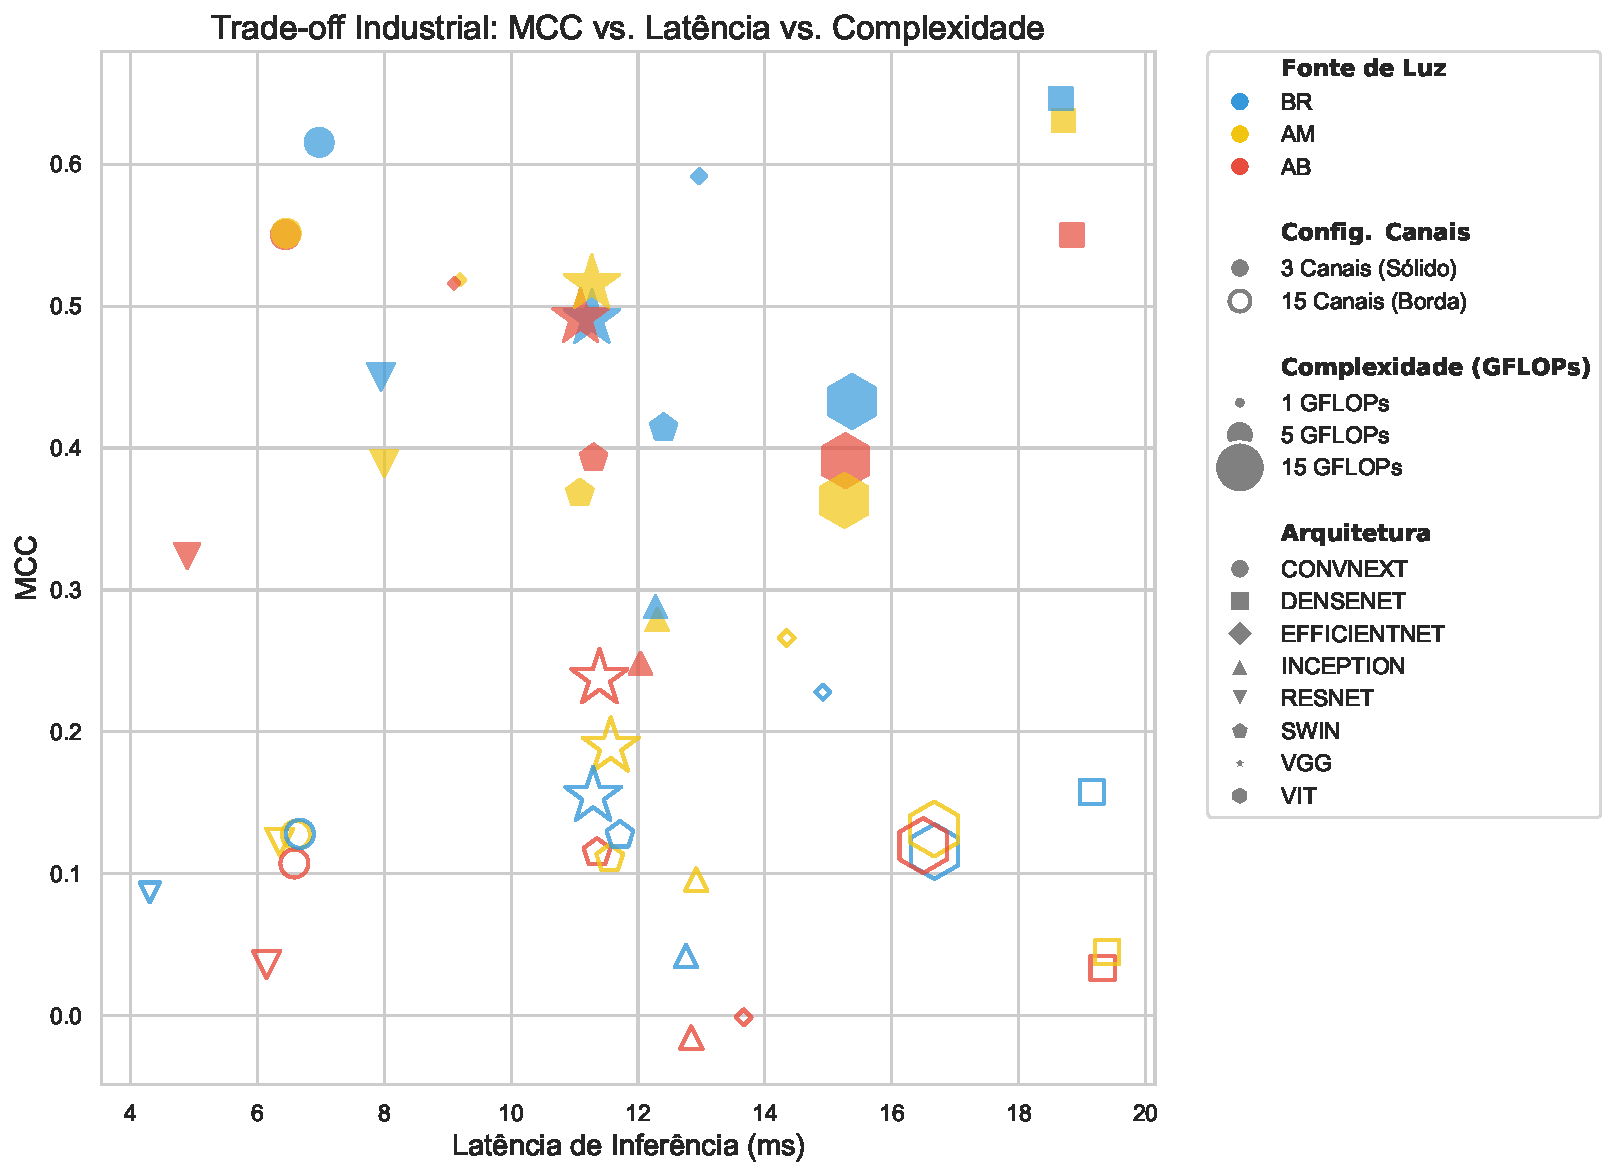
\includegraphics[width=1.0\textwidth]{images/efficiency_tradeoff_full.pdf}
  \legend{Fonte: Do autor (2026).}
\end{figure}

Para quantificar com rigor estatístico o \textit{trade-off} observado na Figura \ref{fig:efficiency_tradeoff}, mediu-se a distribuição completa de latência de inferência para as 8 arquiteturas na versão RGB/BR, ao longo de todo o conjunto de teste retido ($N = 1.578$ \textit{patches}), em lote unitário sobre entrada $224 \times 224$ no mesmo hardware (Apple M3, \textit{backend} MPS). A Tabela \ref{tab:latency_distribution} apresenta a média, o desvio padrão e os percentis 95 e 99 (que caracterizam o pior cenário típico, sem serem \textit{outliers} extremos) para cada arquitetura.

\begin{table}[!h]
    \centering
    \begin{threeparttable}
    \caption{Distribuição de Latência de Inferência por Patch (RGB/BR, $N=1.578$).}
    \label{tab:latency_distribution}
    \begin{tabular}{lrrrrrr}
\toprule
Arquitetura & Média (ms) & Desvio (ms) & Mín (ms) & Máx (ms) & P95 (ms) & P99 (ms) \\
\midrule
\textbf{CONVNEXT} & \textbf{6,44} & \textbf{0,23} & \textbf{6,21} & \textbf{12,97} & \textbf{6,84} & \textbf{7,09} \\
RESNET & 7,87 & 0,45 & 7,40 & 17,77 & 8,66 & 9,10 \\
SWIN & 11,26 & 0,76 & 10,43 & 29,09 & 12,08 & 13,28 \\
VGG & 11,29 & 0,14 & 11,12 & 15,48 & 11,44 & 11,56 \\
INCEPTION & 11,98 & 0,37 & 11,37 & 16,55 & 12,53 & 13,26 \\
EFFICIENTNET & 12,98 & 0,46 & 12,23 & 16,01 & 13,74 & 14,96 \\
VIT & 15,29 & 0,35 & 14,92 & 27,28 & 15,62 & 16,05 \\
\textbf{DENSENET} & \textbf{19,04} & \textbf{1,73} & \textbf{17,79} & \textbf{63,05} & \textbf{20,49} & \textbf{24,66} \\
\bottomrule
\end{tabular}
    \begin{tablenotes}
            \small
            \item[] Fonte: Do autor (2026).
            \item[] Nota: medições em Apple M3 (\textit{backend} MPS), lote unitário, entrada $224 \times 224$; valores comparativos entre arquiteturas, não uma garantia de latência absoluta em hardware industrial dedicado.
        \end{tablenotes}
        \end{threeparttable}
\end{table}

A \textbf{ConvNeXt-Tiny} confirma a estabilidade observada na média ($6,44$ ms), mantendo o P99 em apenas $7,09$ ms --- uma margem estreita entre o caso típico e o pior caso, favorável à operação em esteiras de alta cadência. Já a \textbf{DenseNet-121}, apesar do MCC comparável, apresenta P99 de $24,66$ ms, mais de três vezes o pior caso da ConvNeXt, o que reforça sua menor adequação a cenários industriais de fluxo contínuo.

Conclui-se, portanto, que a \textbf{ConvNeXt (RGB/BR)} representa a solução de maior valor prático e viabilidade corporativa para a automação da classificação do algodão, entregando o balanço definitivo entre assertividade diagnóstica e rendimento operacional.
